% Teste de uma tabela:

% \begin{table}[htb]
% 	% Título de tabelas sempre aparecem antes da tabela
% 	\textsf{\caption{Tabela sem sentido}}
% 	\center
% 	{
% 		\begin{tabular}{l|l}
% 			\hline
% 			Titulo Coluna 1   & Título Coluna 2\\
% 			\hline
% 			X                 & Y\\
% 			X                 & W\\
% 			\hline
% 		\end{tabular}
% 	}
% 	\label{tab:TabelaSemSentido}
% \end{table}
% 
% $Referência à tabela definida no início: \ref{tab:TabelaSemSentido}

% \begin{figure}[htb]
% 	\centering
%   	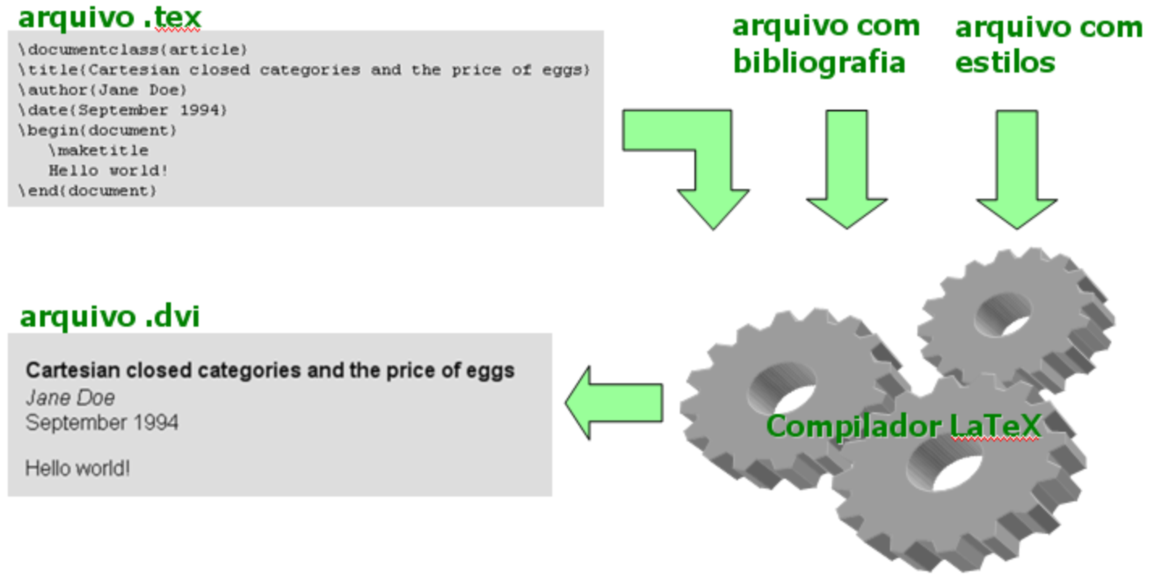
\includegraphics[scale=7.0]{Imagens/FiguraTeste.png}
%   	\textsf{\caption{Teste de uma figura em formato .png}}
%   	\label{fig:FiguraTeste}
% \end{figure}

% Referenciamento da figura inserida na seção anterior: \ref{fig:FiguraTeste}

% \simb[$\lambda$ (algum símbolo)]{$\lambda$}

% \abrv[UFRN -- Universidade Federal do Rio Grande do Norte]{UFRN}

% \cite{siri} é um programa.
% 
% Na tese de Doutorado de Paquete \cite{PaquetePhD}, discute-se sobre algoritmos de busca local estocásticos aplicados a problemas de Otimização Combinatória considerando múltiplos objetivos. Por sua vez, o trabalho de \cite{KnowlesBoundedLebesgue}, publicado nos anais do IEEE CEC de 2003, mostra uma técnica de arquivamento também empregada no desenvolvimento de algoritmos evolucionários multi-objetivo, trabalho esse posteriormente estendido para um capítulo de livro dos mesmos autores \cite{KnowlesBoundedPareto}. Por fim, no relatório técnico de \citeonline{Jaszkiewicz}, fala-se sobre um algoritmo genético híbrido para problemas multi-critério, enquanto no artigo de jornal de Lopez \textit{et al.} \cite{LopezPaqueteStu} trata-se do \textit{trade-off} entre algoritmos genéticos e metodologias de busca local, também aplicados no contexto multi-critério e relacionado de alguma forma ao trabalho de Jaszkiewicz (\citeyear{Jaszkiewicz}).
% 
% Outros exemplos relacionados encontram-se em \cite{Silberschatz} (livro), \cite{DB2XML} (referência da Web) e \cite{Angelo} (dissertação de Mestrado).

% note        = "http://www.w3.org/TR/2010/REC-speech-synthesis11-20100907/",
% Como referenciar:

% % Tese de Doutorado
% @PHDTHESIS{PaquetePhD,
%   AUTHOR = {L.~Paquete},
%   TITLE = {Stochastic Local Search Algorithms for Multiobjective Combinatorial
% Optimization Problems: Methods and Analysis},
%   SCHOOL = {Techniche Universit\"at Darmstadt},
%   YEAR = {2005}
% }
% 
% 
% % Relatorio tecnico
% @TechReport{Jaszkiewicz,
% AUTHOR={ Andrzej Jaszkiewicz},
% TITLE={Genetic local search for multiple objective combinatorial optimization},
% YEAR=1998,
% INSTITUTION={Institute of Computing Science, Poznan University of Technology},
% NUMBER={RA-014/98}
% }
% 
% % Capitulo de Livro
% @InBook{KnowlesBoundedPareto,
%   author = 	 {Joshua Knowles and David Corne},
%   editor = 	 {X. Gandibleux and M. Sevaux and K. S\"orensen and V. \relax{T'Kindt}},
%   title = 	 {Metaheuristics for Multiobjective Optimisation},
%   chapter = 	 {Bounded {P}areto Archiving: Theory and Practice},
%   publisher = 	 {Springer},
%   year = 	 {2004},
%   volume = 	 {535},
%   series = 	 {Lecture Notes in Economics and Mathematical Systems},
%   pages = 	 {39--64},
%   OPTannote = 	 {ISBN: 3-540-20637-X }
% }
% 
% 
% % Artigo em anais de congresso
% @InProceedings{KnowlesBoundedLebesgue,
%   author = 	 {Joshua D. Knowles and David W. Corne and Mark Fleischer},
%   title = 	 {Bounded Archiving using the {L}ebesgue Measure},
%   booktitle = 	 {Proceedings of the IEEE Congress on Evolutionary Computation},
%   pages = 	 {2490--2497},
%   year = 	 {2003},
%   publisher = {IEEE Press}
% }
% 
% 
% % Artigo de jornal
% @Article{LopezPaqueteStu,
%   AUTHOR = { Manuel L{\'o}pez-Ib{\'a}{\~n}ez  and  Lu\'is Paquete  and  Thomas St{\"u}tzle },
%   TITLE = {Hybrid Population-based Algorithms for the
%                   Bi-objective Quadratic Assignment Problem},
%   JOURNAL = {Journal of Mathematical Modelling and Algorithms},
%   YEAR = 2006,
%   VOLUME = 5,
%   NUMBER = 1,
%   PAGES = {111--137}
%  }
%  
%  
% % Livro
% @Book{Silberschatz,
%   author =       {Silberschatz, Abraham and
%                   Korth, Henry F. and
%                   Sudarshan, S.},
%   title =        {Database system concepts},
%   publisher =    {McGraw-Hill},
%   year =         {2002},
%   edition =      {4th},
%   address = {Boston}
% }
% 
% %Referencia da Web
% @Misc{DB2XML,
%     author =     {Volker Turau},
%     title =      {DB2XML 1.4: {Transforming} relational databases into {XML} documents},    
%     month =     Oct,
%     year =   {2001},
%     note = {Out., 2001. Disponível em: <\url{http://www.informatik.fh-wiesbaden.de/~turau/DB2XML/index.html}>. Acesso em Abril 9, 2004},
% }
% 
% 
% % Dissertação de Mestrado
% @MasterThesis{Angelo,
%   AUTHOR =       "Angelo Agra",
%   TITLE =        "Implementação de uma Proposta para Atualização de Bancos de Dados através de Visões",
%   SCHOOL =       "Instituto de Informática, UFRGS",
%   YEAR =         "2004",
%   type =         "{Projeto de Diplomação}",
%   address =      "Porto Alegre, RS, Brasil",
%   month =        Jul
% }